\documentclass{CompilerAssignment}
\usepackage{multicol}
\usepackage{multirow}
\usepackage{longtable}
\usepackage{tikz}
\usepackage{enumitem}

\newcommand{\mbfa}{\mathbf{a}}
\newcommand{\bfa}{\textbf{a}}
\newcommand{\first}{\text{FIRST}}
\newcommand{\follow}{\text{FOLLOW}}

\setlength{\columnseprule}{0.5pt}

\title{Assignment 5}

\begin{document}

\maketitle

\section{Exercise 1}

\begin{enumerate}
    \item $(3 + 4) * (5 + 6) \mathbf{n}.$
    \begin{center}
        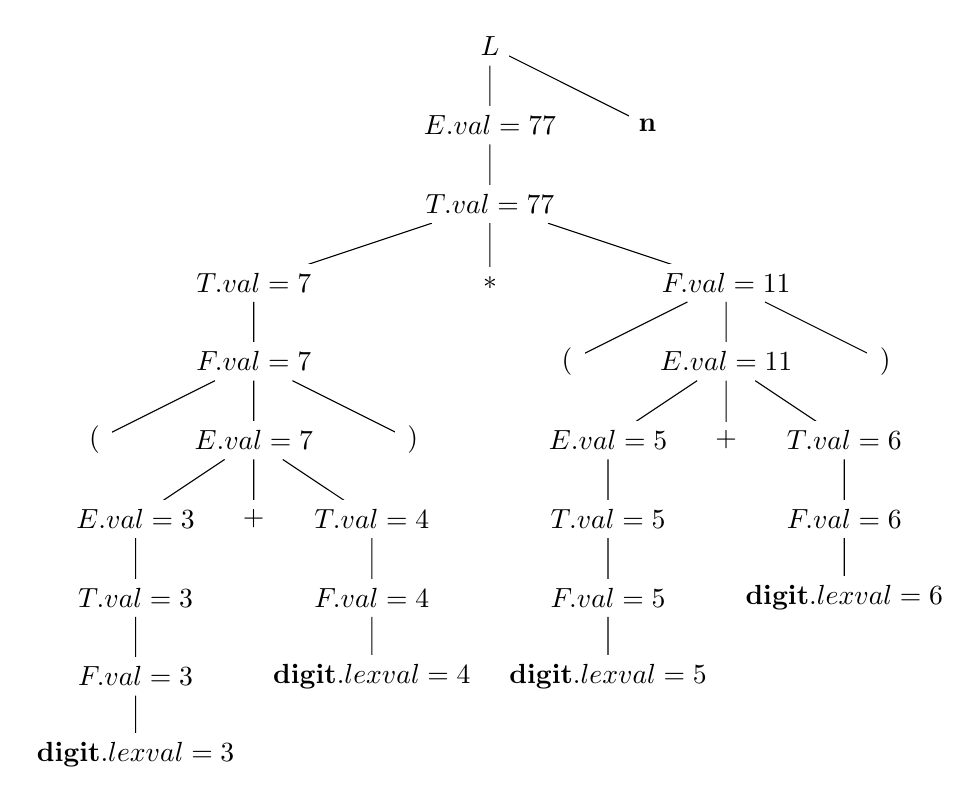
\begin{tikzpicture}
            \draw
            (0, 0) node[fill=white](L) {$L$}
            (L) -- ++(0, -1) node[fill=white](E) {$E.val=77$}
            (L) -- ++(2, -1) node[fill=white] {$\mathbf{n}$}
            (E) -- ++(0, -1) node[fill=white](T) {$T.val=77$}
            (T) -- ++(-3, -1) node[fill=white](T1) {$T.val=7$}
            (T) -- ++(0, -1) node[fill=white] {$*$}
            (T) -- ++(3, -1) node[fill=white](F) {$F.val=11$}
            (T1) -- ++(0, -1) node[fill=white](F1) {$F.val=7$}
            (F1) -- ++(-2, -1) node[fill=white] {$\left( \right.$}
            (F1) -- ++(0, -1) node[fill=white](E1) {$E.val=7$}
            (F1) -- ++(2, -1) node[fill=white] {$\left. \right)$}
            (E1) -- ++(-1.5, -1) node[fill=white](E2) {$E.val=3$}
            (E1) -- ++(0, -1) node[fill=white] {$+$}
            (E1) -- ++(1.5, -1) node[fill=white](T2) {$T.val=4$}
            (E2) -- ++(0, -1) node[fill=white](T3) {$T.val=3$}
            (T2) -- ++(0, -1) node[fill=white](F2) {$F.val=4$}
            (T3) -- ++(0, -1) node[fill=white](F3) {$F.val=3$}
            (F) -- ++(-2, -1) node[fill=white] {$\left( \right.$}
            (F) -- ++(0, -1) node[fill=white](E3) {$E.val=11$}
            (F) -- ++(2, -1) node[fill=white] {$\left. \right)$}
            (E3) -- ++(-1.5, -1) node[fill=white](E4) {$E.val=5$}
            (E3) -- ++(0, -1) node[fill=white] {$+$}
            (E3) -- ++(1.5, -1) node[fill=white](T4) {$T.val=6$}
            (E4) -- ++(0, -1) node[fill=white](T5) {$T.val=5$}
            (T4) -- ++(0, -1) node[fill=white](F4) {$F.val=6$}
            (T5) -- ++(0, -1) node[fill=white](F5) {$F.val=5$}
            (F4) -- ++(0, -1) node[fill=white](d4) {$\mathbf{digit}.lexval=6$}
            (F5) -- ++(0, -1) node[fill=white](d5) {$\mathbf{digit}.lexval=5$}
            (F2) -- ++(0, -1) node[fill=white](d2) {$\mathbf{digit}.lexval=4$}
            (F3) -- ++(0, -1) node[fill=white](d3) {$\mathbf{digit}.lexval=3$};
        \end{tikzpicture}
    \end{center}
    \newpage
    \item $1 * 2 * 3 * (4 + 5) \mathbf{n}.$
    \begin{center}
        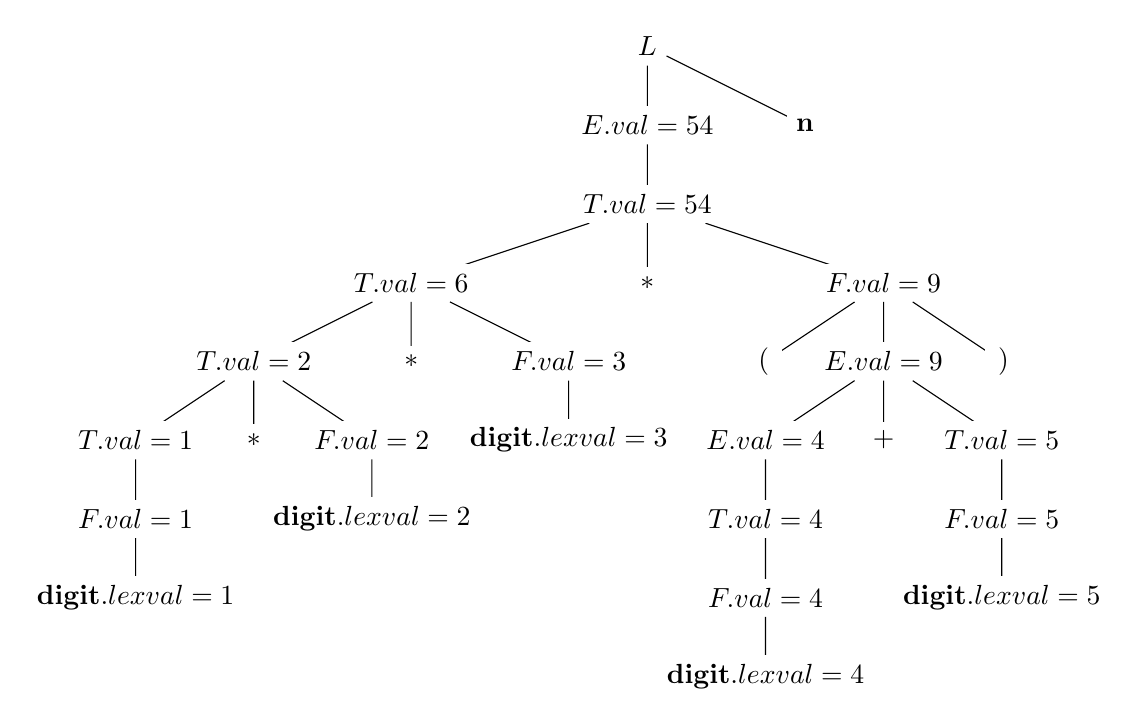
\begin{tikzpicture}
            \draw
            (0, 0) node[fill=white](1) {$L$}
            (1) -- ++(0, -1) node[fill=white](2) {$E.val=54$}
            (1) -- ++(2, -1) node[fill=white] {$\mathbf{n}$}
            (2) -- ++(0, -1) node[fill=white](3) {$T.val=54$}
            (3) -- ++(-3, -1) node[fill=white](4) {$T.val=6$}
            (3) -- ++(0, -1) node[fill=white] {$*$}
            (3) -- ++(3, -1) node[fill=white](5) {$F.val=9$}
            (4) -- ++(2, -1) node[fill=white](6) {$F.val=3$}
            (4) -- ++(0, -1) node[fill=white](7) {$*$}
            (4) -- ++(-2, -1) node[fill=white](8) {$T.val=2$}
            (6) -- ++(0, -1) node[fill=white](d6) {$\mathbf{digit}.lexval=3$}
            (5) -- ++(-1.5, -1) node[fill=white] {$\left( \right.$}
            (5) -- ++(0, -1) node[fill=white](9) {$E.val=9$}
            (5) -- ++(1.5, -1) node[fill=white] {$\left. \right)$}
            (9) -- ++(-1.5, -1) node[fill=white](10) {$E.val=4$}
            (9) -- ++(0, -1) node[fill=white] {$+$}
            (9) -- ++(1.5, -1) node[fill=white](11) {$T.val=5$}
            (10) -- ++(0, -1) node[fill=white](12) {$T.val=4$}
            (11) -- ++(0, -1) node[fill=white](17) {$F.val=5$}
            (12) -- ++(0, -1) node[fill=white](18) {$F.val=4$}
            (17) -- ++(0, -1) node[fill=white](d17) {$\mathbf{digit}.lexval=5$}
            (18) -- ++(0, -1) node[fill=white](d18) {$\mathbf{digit}.lexval=4$}
            
            (8) -- ++(-1.5, -1) node[fill=white](13) {$T.val=1$}
            (8) -- ++(0, -1) node[fill=white](14) {$*$}
            (8) -- ++(1.5, -1) node[fill=white](15) {$F.val=2$}
            (13) -- ++(0, -1) node[fill=white](16) {$F.val=1$}
            (15) -- ++(0, -1) node[fill=white](d15) {$\mathbf{digit}.lexval=2$}
            (16) -- ++(0, -1) node[fill=white](d16) {$\mathbf{digit}.lexval=1$};
        \end{tikzpicture}
    \end{center}

    \item $(9 + 8 * (7 + 6) + 5) * 4 \mathbf{n}.$
    \begin{center}
        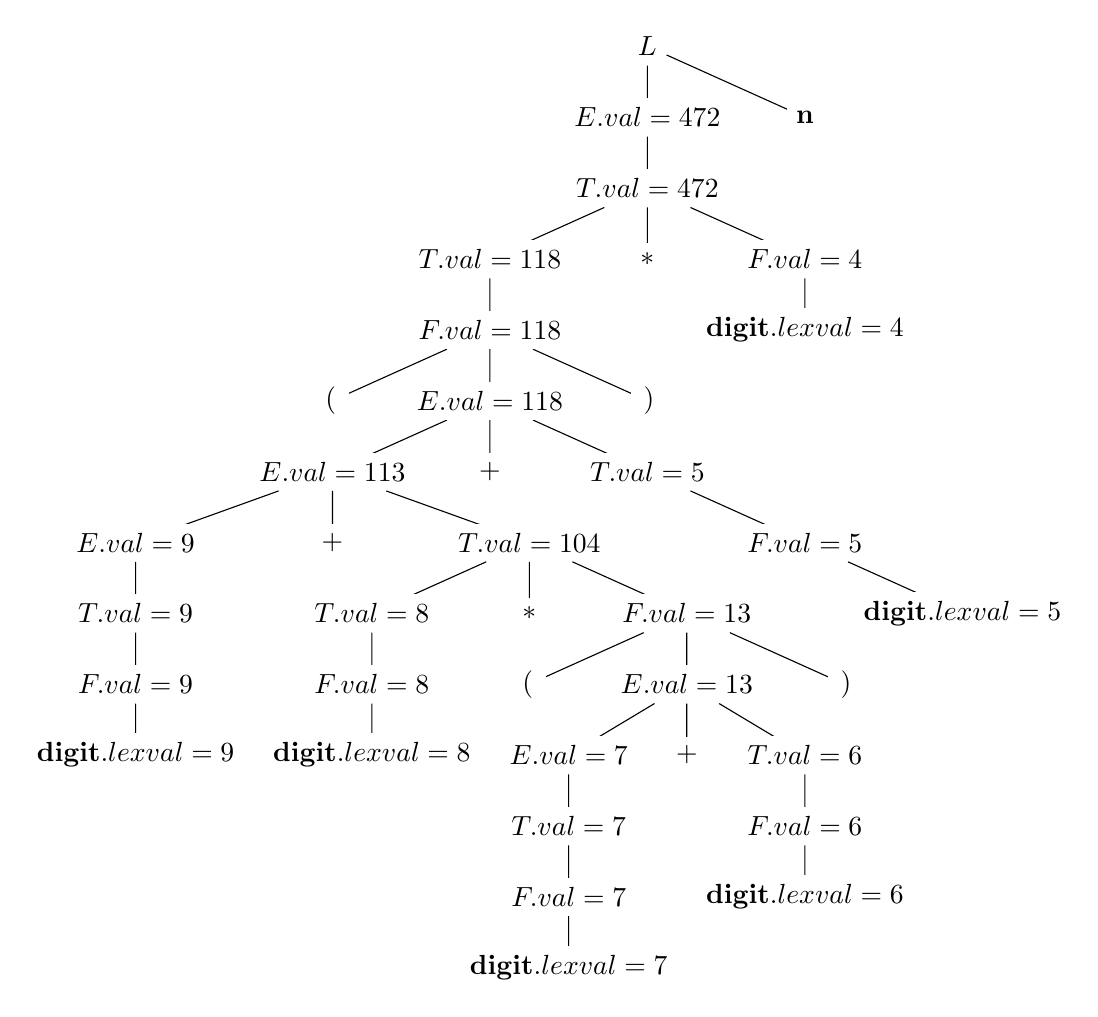
\begin{tikzpicture}
            \draw
            (0, 0) node[fill=white](1) {$L$}
            (1) -- ++(0, -0.9) node[fill=white](2) {$E.val=472$}
            (1) -- ++(2, -0.9) node[fill=white] {$\mathbf{n}$}
            (2) -- ++(0, -0.9) node[fill=white](3) {$T.val=472$}
            (3) -- ++(-2, -0.9) node[fill=white](4) {$T.val=118$}
            (3) -- ++(0, -0.9) node[fill=white] {$*$}
            (3) -- ++(2, -0.9) node[fill=white](5) {$F.val=4$}
            (4) -- ++(0, -0.9) node[fill=white](6) {$F.val=118$}
            (6) -- ++(-2, -0.9) node[fill=white] {$\left( \right.$}
            (6) -- ++(0, -0.9) node[fill=white](7) {$E.val=118$}
            (6) -- ++(2, -0.9) node[fill=white] {$\left. \right)$}
            (7) -- ++(-2, -0.9) node[fill=white](8) {$E.val=113$}
            (7) -- ++(0, -0.9) node[fill=white] {$+$}
            (7) -- ++(2, -0.9) node[fill=white](9) {$T.val=5$}
            (8) -- ++(-2.5, -0.9) node[fill=white](10) {$E.val=9$}
            (8) -- ++(0, -0.9) node[fill=white] {$+$}
            (8) -- ++(2.5, -0.9) node[fill=white](11) {$T.val=104$}
            (10) -- ++(0, -0.9) node[fill=white](12) {$T.val=9$}
            (12) -- ++(0, -0.9) node[fill=white](13) {$F.val=9$}
            (13) -- ++(0, -0.9) node[fill=white](d13) {$\mathbf{digit}.lexval=9$}
            (11) -- ++(-2, -0.9) node[fill=white](14) {$T.val=8$}
            (11) -- ++(0, -0.9) node[fill=white] {$*$}
            (11) -- ++(2, -0.9) node[fill=white](15) {$F.val=13$}
            (14) -- ++(0, -0.9) node[fill=white](16) {$F.val=8$}
            (16) -- ++(0, -0.9) node[fill=white](d16) {$\mathbf{digit}.lexval=8$}
            (15) -- ++(-2, -0.9) node[fill=white] {$\left( \right.$}
            (15) -- ++(2, -0.9) node[fill=white] {$\left. \right)$}
            (15) -- ++(0, -0.9) node[fill=white](17) {$E.val=13$}
            (17) -- ++(-1.5, -0.9) node[fill=white](18) {$E.val=7$}
            (17) -- ++(0, -0.9) node[fill=white] {$+$}
            (17) -- ++(1.5, -0.9) node[fill=white](19) {$T.val=6$}
            (18) -- ++(0, -0.9) node[fill=white](20) {$T.val=7$}
            (20) -- ++(0, -0.9) node[fill=white](21) {$F.val=7$}
            (21) -- ++(0, -0.9) node[fill=white](d21) {$\mathbf{digit}.lexval=7$}
            (19) -- ++(0, -0.9) node[fill=white](22) {$F.val=6$}
            (22) -- ++(0, -0.9) node[fill=white](d22) {$\mathbf{digit}.lexval=6$}
            (9) -- ++(2, -0.9) node[fill=white](23) {$F.val=5$}
            (23) -- ++(2, -0.9) node[fill=white](d23) {$\mathbf{digit}.lexval=5$}
            (5) -- ++(0, -0.9) node[fill=white](d5) {$\mathbf{digit}.lexval=4$};
        \end{tikzpicture}
    \end{center}
\end{enumerate}

\section{Exercise 2}

There all totoally 10 different topological sorts for the dependency graph.

\begin{enumerate}[label=\arabic*: ]
    \item 1, 2, 3, 4, 5, 6, 7, 8, 9;
    \item 1, 2, 3, 5, 4, 6, 7, 8, 9;
    \item 1, 2, 4, 3, 5, 6, 7, 8, 9;
    \item 1, 3, 2, 4, 5, 6, 7, 8, 9;
    \item 1, 3, 2, 5, 4, 6, 7, 8, 9;
    \item 1, 3, 5, 2, 4, 6, 7, 8, 9;
    \item 2, 1, 3, 4, 5, 6, 7, 8, 9;
    \item 2, 1, 3, 5, 4, 6, 7, 8, 9;
    \item 2, 1, 4, 3, 5, 6, 7, 8, 9;
    \item 2, 4, 1, 3, 5, 6, 7, 8, 9.
\end{enumerate}

\section{Exercise 3}

\begin{table}[!h]
    \centering
    \begin{tabular}{cl|l}
        \hline \hline
        & \textsc{Productions} & \textsc{Semantic Rules} \\ \hline
        1) & $E \rightarrow E_1 + T$ & $ E.type:=\mathrm{float}\ \mathbf{if}\ E_1.type=\mathrm{float}\ \mathbf{else}\ \mathrm{int} $ \\
        2) & $E \rightarrow T$ & $ E.type := T.type $ \\
        3) & $T \rightarrow num.num$ & $ T.type:=\mathrm{float} $ \\
        4) & $T \rightarrow num$ & $ T.type:=\mathrm{int} $\\
        \hline
    \end{tabular}
\end{table}

\end{document}